\documentclass{article}

\usepackage{amsfonts}
\usepackage{amsmath}
\usepackage{amsthm}
\usepackage{graphicx}
\usepackage[colorlinks=true,citecolor=blue,linkcolor=blue,filecolor=blue,urlcolor=blue,pdfborder={0 0 0}]{hyperref}
\usepackage[utf8]{inputenc}
\usepackage{multicol}
\usepackage{natbib}
\usepackage{subcaption}

\title{Nearest Neighbour Methods for Length of Stay Prediction}
\author{
  Tianyu Pu, Irena Koprinska, Kalina Yacef\\
  School of Information Technologies\\
  University of Sydney, NSW, 2006\\
  \texttt{\{tianyu.pu,irena.koprinska,kalina.yacef\}@sydney.edu.au}
  \and
  Michael Dinh\\
  Trauma Services, Royal Prince Alfred Hospital\\
  Sydney, NSW, 2042\\
  \texttt{dinh.mm@gmail.com}
}

\date{\today}

\begin{document}
\maketitle

\renewcommand{\abstractname}{Summary}

\begin{abstract}
Objective:

Materials and methods:

Results:

Conclusions:

Keywords:

\end{abstract}

\section{Introduction}
Hospitals often have limited funding, and therefore managing and utilising
their resources efficiently has always been a priority \cite{Walczak2003}.
One key measurement of hospital activity, health care utilisation and hospital
cost is the patient length of stay \citep{Omachonu2004,Ng2006}.
The length of
stay has been used in a wide variety of medical domains, such as burns
 \citep{Yang2010}, intensive
care \citep{Tu1993,Harper2005,Perez2006,Dybowski1996},
psychiatry \citep{Lowell1997}, and acute pancreatitis \citep{Pofahl1998}, in
order to assist hospitals in allocating beds and other patient management
resources as efficiently as possible. However, given the many different
conditions that hospitals manage, the length of stay of a patient is
not easy to predict \citep{Walczak2003}, especially upon a patient's admission.
Many methods have been explored in the literature, from the realm of statistics
to techniques in data mining, and they have been explored for many different
medical domains.

One of the more well-understood and widely used statistical methods for
predicting the length of stay is \textit{logistic regression} \citep{Tu1996}.
Logistic regression models are straightforward to construct and use via the
help of statistical software packages such as
SAS\footnote{SAS Institute, Cary, NC, USA}, and
also make the contribution of each independent variable to the final
prediction explicit. Thus they are easier to interpret when compared to more
``black box'' approaches such as artificial neural networks \citep{Adams2012}.
A wide variety of other statistical approaches have been proposed, notably:
various scoring systems from univariate analysis \citep{Adams2012,Lavoie2005},
linear regression \citep{Yang2010}, exponential models \citep{Clark2007},
survival analysis \citep{Vasilakis2005}, and Markov
models \citep{Perez2006,Jain1989,Kapadia2000}.

Out of the development of the various statistically-motivated models, data
mining techniques, particularly artificial neural networks,
began to be more widely adopted following a number of
early applications to length of stay prediction in intensive
care \citep{Tu1993,Dybowski1996}, in addition to disease diagnosis and mortality
prediction \citep{Silva2006}. Artificial neural networks are able to detect
complex and non-linear relationships between input and output variables and can
be developed using many different techniques. Much work has been done in using
neural networks to predict patient length of stay in various medical conditions
such as acute pancreatitis \citep{Walczak2003}, gastroenteritis \citep{Ng2006},
surgical intensive care \citep{Buchman1994,Tu1993} and
psychiatry \citep{Lowell1997}. Other data mining techniques have also been
applied, such as support vector machines and tree-based
methods \citep{Harper2005}.

One of the major drawbacks of sophisticated data mining techniques is the high
level of difficulty required in interpreting their predictions and the factors
affecting those predictions. This is
particularly true of artificial neural networks and the state-of-the-art
support vector machine, which are able to achieve very high accuracy but can be
non-intuitive to understand. Medical domain experts who use the predictions of
trained learning algorithms need to understand how the algorithm reached its
decision before they are able to confidently use it to aid their clinical
decision-making.

In this paper we present the application of nearest neighbour methods
in predicting the length of stay category for patients admitted to a trauma
ward. The categories are \textit{less than or equal to 2 days} or
\textit{greater than 2 days}, which have been used in previous work on length
of stay prediction in the same medical domain \citep{Dinh2013a}.
Nearest neighour methods have not been studied in predicting the length of stay,
and we believe they are much more intuitive to
understand than techniques such as support vector machines.
Additionally, they can be adjusted to suit particular medical domains by
changing their similarity function. We compare the performance of the basic
nearest neighbour algorithm, as well as an extension (K*), against the
performance
of previous work which used logistic regression. We also propose a novel
extension to the standard nearest neighbour algorithm, Ranked Distance, and
test its performance against the other classifiers. In addition, we apply a
range of feature selection methods and systematically investigate the effect
of discretisation, as they have not been
thoroughly studied in existing work. Finally, we compare the performance of
these with the state-of-the-art support vector machines and the
commonly-used artificial neural networks.

We found that the standard nearest neighbour classifier using only 1 nearest
neighbour achieved a ten-fold cross-validated accuracy of 77.81\%, the highest
out of all the methods. This is an improvement of 2.75\% over previous work
carried out by Dinh et al. \citep{Dinh2013a} using the same data set. Also, the
nearest neighbour classifiers almost always outperformed the logistic
regression, support vector machines and neural networks when the number of
features was gradually reduced. This means that predictions are able to be made
more quickly, and will also be more intuitive to interpret and understand for
physicians.

In Section \ref{sec:nn}, we outline the basics of nearest neighbour
classification and describe both the existing K* extension and our proposed
extension, Ranked Distance. Section \ref{sec:features} outlines the feature
selection methods we used. Section \ref{sec:eval} describes the method used
to evaluate the performance of these classifiers, and Section \ref{sec:results}
proceeds to discuss the results. We present concluding remarks in Section
\ref{sec:conclusions}.

\section{Nearest Neighbour Classification}
\label{sec:nn}

\subsection{Basic Algorithm}
The $k$-nearest neighbour ($k$-NN) classifier is an example of an
\textit{instance-based} learning algorithm. This is because it does not attempt
to deduce or
generalise a relationship between the features and the class: it simply stores
all training examples and classifies an unseen example by finding the $k$
``nearest'' examples (or \textit{instances}) and assigning the majority class
to the new example. In the simplest form of the algorithm, $k$ is chosen to be
1 and the Euclidean distance is used to measure the closeness of neighbours:
\begin{equation*}
\mathrm{Distance} = \sqrt{(x_1-y_1)^2 + (x_2-y_2)^2 + \ldots + (x_n-y_n)^2}
\end{equation*}
where $x_i,y_i$ are the values of the $i$-th feature for two different feature
vectors (or instances).

\subsection{Normalisation}
$k$-NN allows all features to be taken
into account equally when classifying a new example. However, since feature
values often span different ranges and units of measurement, a particularly
large range of values for a feature would contribute much more to the distance
than another feature that spans a lower set of values.
To avoid this, it is important to \textit{normalise} the
values of each numeric feature before using $k$-NN: for each feature $i$, we
calculate the normalised value of the feature for each training example. This
is done using the following relationship:
\begin{equation}
\label{eq:normalise}
a_i = s\left(\dfrac{v_i - \mathrm{min }v_i}{\mathrm{max }v_i - \mathrm{min }v_i}\right) + t
\end{equation}
where $a_i$ is the normalised feature value, $v_i$ is the actual value in the
data set, max $v_i$ and min $v_i$ are taken over all training examples, $s$ is
a scaling factor and $t$ indicates how much to translate the range by. If $s=1$
and $t=0$, then the range of normalised values will be in $[0,1]$.

\subsection{Existing and Proposed Extensions}
There have been many extensions proposed to the $k$-NN algorithm described
above. These usually seek to find a more suitable distance metric for the
problem domain at hand, or to reduce the storage requirements of the original
$k$-NN algorithm (since the classifier makes no attempt to generalise from the
examples, all of them must be stored).
We will focus on two algorithms that extend the standard Euclidean distance:
K* and our proposed approach, Ranked Distance Nearest Neighbour.

\subsubsection{K*: Instance-based Classifier with Entropic Distance Function}
Cleary and Trigg developed K*, an instance-based classifier that uses entropy
to measure the distances between instances \cite{Cleary1995}. They consider
the distance between two instances to be the complexity of transforming one
into another. Define a sequence of transformations on an instance:
\begin{equation*}
\bar{t}(a) = t_n(t_{n-1}(\ldots t_1(a)\ldots)), \bar{t} \in T
\end{equation*}
where $\bar{t} = t_1,\ldots,t_n$. We can define a probability function $p$
that gives the probabilities of these transformations occurring, and then we
can define a probability function that gives the probabilities of all paths
(transformations) from example $a$ to $b$:
\begin{equation*}
P^*(b|a) = \sum_{\bar{t}\in T:\bar{t}(a)=b} p(\bar{t})
\end{equation*}
Within this framework, we can define transformations for both real-valued and
categorical features, which allows K* to work with all types of features.
The K* function is then defined as:
\begin{equation*}
K^*(b|a) = -\mathrm{log}_2P^*(b|a)
\end{equation*}

To calculate the probability of an instance $a$ being in a class $C$, we sum
the probabilities from $a$ to each instance of $C$, and repeat for each class.
The predicted class will be the one with the highest probability:
\begin{equation*}
P^*(C|a) = \sum_{b\in C} P^*(b|a)
\end{equation*}

We use K* as a comparison to the basic NN algorithm and also as a comparison
to our proposed Ranked Distance Nearest Neighbour algorithm. Additionally,
K* has not been yet been applied in predicting LOS, and its performance in this
domain is worth investigating.

\subsubsection{Ranked Distance Nearest Neighbour}
\paragraph{Intuition.}
As we mentioned earlier, all features are considered equally in a $k$-NN
classifier, which implies that all features are equally important in predicting
the class. In practice, however, this is not always the case: to predict the
LOS of a trauma patient, the severity of their injury should affect the final
LOS more than whether or not they can speak English (which could be just two
of many features that are recorded about a patient). Our contribution is a
new NN algorithm that uses a modified distance function which takes into
account the relative importance of all features called Ranked Distance
Nearest Neighbour (RD).

\paragraph{Mathematical formulation.}
Given two instances $\mathbf{x} = (x_1,x_2,\ldots,x_n)$ and
$\mathbf{y} = (y_1,y_2,\ldots,y_n)$, the distance between them is given by:
\begin{equation*}
\mathrm{Distance} = \sum_{i=1}^n w_i |x_i-y_i|
\end{equation*}
where the $w_i$s weight the contribution of the $i$-th feature to the overall
distance that is computed by the $k$-NN algorithm. We assume that all feature
values have been normalised, as described above.

\paragraph{Assignment of weights.}
The weights $w_i$ can be tuned to match the particular problem that is being
investigated. For our LOS classification problem, we will consider one way
of weighting features.
First, we compute the correlation coefficients as described in the point above.
This gives us a ranking of the importance of each feature to the prediction of
the class, with 1 being the highest rank (indicating the most importance) and
$n$ being the lowest rank (indicating the least importance).
Instead of using the values of the correlation directly to weight
the distance contribution of each feature, we specify a function:
\begin{equation*}
f : \mathrm{Rank} \rightarrow \mathbb{R}, \mathrm{Rank} \in \{1,2,\ldots,n\}
\end{equation*}
that describes
how the weights of the features vary with the rank. This function should
inituitively be non-increasing and should produce lower values when the rank
number is greater, meaning that less important features have a lower weight
in the distance calculation.
Note that choosing $f(\mathrm{Rank}) = k$ for any non-zero constant $k$
results in all features contributing equally to the distance calculation.
We will use $f(\mathrm{Rank}) = \frac{1}{\mathrm{Rank}^c}$, where
$c$ varies from 0 to 1.

\section{Feature Selection}
\label{sec:features}
Here we introduce the feature selection algorithms we evaluate in our work.
Several of these have not been investigated in previous work on LOS prediction.
The role of feature selection is to reduce the number of attributes taken into
consideration by a learning algorithm, which improves running speed and can
make the resulting learned relationship easier to understand. We used both
automatic and manual methods of selecting features.

\subsection{Automatic Selection}
Automatic feature selection involves calculating the ``relevance'' of each
feature to predicting the class and only keeping features for use in training
if their relevance is above some threshold. We consider the Pearson correlation
coefficient, information gain and the wrapper approach.

\subsubsection{Pearson Correlation Coefficient}
The Pearson correlation coefficient measures the degree of linear correlation
between two variables. It is always in the range $[-1,1]$, where $-1$ is total
negative correlation, 0 is no (linear) correlation, and 1 is total positive
correlation. We compute the Pearson correlation between each feature and the
class using:
\begin{equation*}
r_i = \dfrac{\sum_{i=1}^m (x_i-\bar{x})(c-\bar{c})}{\sqrt{(\sum_{i=1}^m x_i-\bar{x})(\sum_{i=1}^m c-\bar{c})}}
\end{equation*}
where $m$ is the number of training examples, $x_i$ is the value of feature
$i$, and $\bar{x}$ and $\bar{c}$ are the arithmetic averages of the feature
values and the class values respectively.

\subsubsection{Information Gain}
We can also measure the information gain (IG) of each feature as follows.
If we have a class $C$ and a feature $F$, the entropy of the
class before and after observing the feature is:
\begin{equation*}
\begin{aligned}
& \mathrm{entropy}(C) = - \sum_{c \in C} p(c) \mathrm{log}_2 p(c) \\
& \mathrm{entropy}(C|F) = - \sum_{f \in F} p(f) \sum_{c \in C} p(c|f) \mathrm{log}_2 p(c|f)
\end{aligned}
\end{equation*}
The decrease in entropy reflects the gain in information provided by the
feature and is given by:
\begin{equation*}
IG(C|F) = \mathrm{entropy}(C) - \mathrm{entropy}(C|F)
\end{equation*}

We can compute the IG for each feature and then select subsets of features that
are greater than some threshold we specify, similar to the correlation
coefficient method of feature selection. We choose a similar set of thresholds
because of the high numbers of features with very low information gain.

\subsubsection{Wrapper-based Feature Selection}
The feature selection methods described above (Pearson correlation and IG) have
been described as \textit{filter} approaches to
attribute selection, because the feature set is reduced \textit{before} it
is given to the learning algorithm.
Kohavi and John proposed another approach, the \textit{wrapper} approach:
instead of performing feature selection independently of the learning
algorithm using some measure of ``relevance,''
the learning algorithm itself is used to evaluate the goodness of
subsets of features \cite{Kohavi1997}. 

A key advantage of the wrapper approach is that the selected feature sets are
specifically tailored to a learning algorithm, which ensures the best
performance of that algorithm given the data set. However, wrapper approaches
can also be prohibitively slow if the data or feature sets are large and the
chosen learning algorithm expensive to train (such as support vector machines
and multi-layer perceptrons). We will evaluate the use of C4.5 decision trees
in selecting features using the wrapper approach.
Using decision trees to select features is relatively fast as due to the
divide and conquer nature of the learning algorithm, and the tendency of the
trees to select fewer features for learning than other algorithms.
Wrapper methods search for the best subset of features and do not require a
threshold to discard attributes.

\subsection{Manual Selection}
All of the above automatic feature selection methods use some notion of
``relevance,'' such as information gain or linear correlation,
in order to determine the best subset of features to select.
Depending on the problem at hand, these definitions of relevance may or may
not work well with the data. In the LOS prediction literature, studies
have enlisted the help of medical domain experts to assist in feature
selection, due to their experience and understanding of the underlying
problem and the effect of the features on the outcome. It will therefore be
worthwhile to compare the performance of classifiers using features selected
automatically and manually.

\subsubsection{Domain Expert Selection}
Consultation with a domain expert yielded a feature set that we
use to compare with the baseline and with the other automatic methods.

\subsection{Baseline Feature Set}
The key previous work on trauma LOS prediction was by Dinh et. al.
\cite{Dinh2013a}, who used a specific feature set from the data set that we
use. We would like to use the features they selected as a baseline for
evaluating the other feature selection methods we describe.

\section{Evaluation}
\label{sec:eval}
\subsection{Data Set}
The data set used consisted of trauma registry data from the trauma centre
at the Royal Prince Alfred Hospital, a major trauma centre in New South Wales,
Australia. It covered all adult (age 15 and over) inpatient admissions to the
trauma centre from 2007--2011. 
All patients were first admitted to the trauma ward until discharged
or transferred to an appropriate unit within the hospital. A single trained
data manager recorded a variety of attributes about the admitted patient,
such as age, gender, blood pressure, mechanism of injury and body regions
that were injured.

There were 2546 patient records in the data set we received, comprising of 79
features, one of which was the target variable \texttt{los48}.
\texttt{los48} was a binary variable -- that is, it could only take two
values, 0 or 1 -- with 1 indicating that the patient stayed two days or less,
and 0 indicating a stay of longer than 2 days.

\subsection{Preprocessing}
The data set was cleaned by correcting spelling and punctuation
inconsistencies and removing extraneous whitespace. Examples which had missing
values for at least one feature were removed, in line with previous work on the
same data set.

Continuous-valued features were then normalised into the $[0,1]$ range as
described in Section \ref{sec:nn} above, substituting $s=2$ and $t=-1$ into
Equation \ref{eq:normalise}. These continuous features were then discretised
using Fayyad and Irani's method of supervised discretisation
\citep{Fayyad1993}. We kept both the original data set (normalised, without
discretisation) and the discretised (and normalised) data set for comparison.

\subsection{Classification Algorithms}
We tested the performance of
support vector machines (SVMs), multi-layer perceptrons (MLPs), $k$-nearest
neighbour with 1
and 20 nearest neighbours, K* and logistic regression (LR), as well as our
proposed
Ranked Distance Nearest Neighbour (RD) -- a total of 7 different classifiers.

\subsection{Experimental Setup and Procedure}
The steps that we took to evaluate the performance of the various classifiers
and feature selection methods were:
\begin{enumerate}
\item For both the discretised and non-discretised data set, we trained all 7
classifiers without feature selection. Evaluation was performed using ten runs
of \textit{ten-fold stratified cross-validation}.
\item Then, for each data set, we evaluated the effect of the 3 automatic
feature
selection methods on each of the 7 classifiers listed above, giving us 21
configurations for the discretised and non-discretised data set.
\item In order to ensure that the baseline in the literature was comparable
to our work, we used the baseline features and applied their method, logistic
regression, to obtain a measure of performance on the non-discretised data set.
We also evaluated this feature set against the rest of the 6 classifiers, and
repeated this using the discretised data.
\item Additionally, the expert-selected features were tested against all 7
classifiers, with both the discretised and non-discretised data.
\item Paired $t$-tests for statistical significance were carried out to
determine whether or not discrepancies in performance were significant.
\end{enumerate}

\section{Results and Discussion}
\label{sec:results}

\subsection{Overall Performance}
The best accuracy was 77.81\%, achieved using the $k$-NN algorithm
with 1 nearest neighbour, a discretised data set, and feature selection using a
C4.5 wrapper. The best AUC of 0.846 was achieved using logistic regression with
features selected by a correlation coefficient threshold of 0.1, again
using the discretised data set.

\begin{figure*}[htbp]
\begin{subfigure}{.50\textwidth}
\includegraphics[width=\textwidth]{results/tr-nofs-acc.eps}
\caption{}
\label{}
\end{subfigure}%
\begin{subfigure}{.57\textwidth}
\includegraphics[width=\textwidth]{results/tr-nofs-auc.eps}
\caption{}
\label{}
\end{subfigure}

\begin{subfigure}{.50\textwidth}
\includegraphics[width=\textwidth]{results/tr-dinh-acc.eps}
\caption{}
\label{}
\end{subfigure}%
\begin{subfigure}{.57\textwidth}
\includegraphics[width=\textwidth]{results/tr-dinh-auc.eps}
\caption{}
\label{}
\end{subfigure}

\begin{subfigure}{.50\textwidth}
\includegraphics[width=\textwidth]{results/tr-expert-acc.eps}
\caption{}
\label{}
\end{subfigure}%
\begin{subfigure}{.57\textwidth}
\includegraphics[width=\textwidth]{results/tr-expert-auc.eps}
\caption{}
\label{}
\end{subfigure}

\begin{subfigure}{.50\textwidth}
\includegraphics[width=\textwidth]{results/tr-wrapper-acc.eps}
\caption{}
\label{}
\end{subfigure}%
\begin{subfigure}{.57\textwidth}
\includegraphics[width=\textwidth]{results/tr-wrapper-auc.eps}
\caption{}
\label{}
\end{subfigure}
\caption[]{Comparison of accuracy and AUC between classifiers for each non-threshold feature selection method, grouped by whether or not discretisation was applied.}
\label{}
\end{figure*}

\begin{figure}[htbp]
\begin{subfigure}{1.1\textwidth}
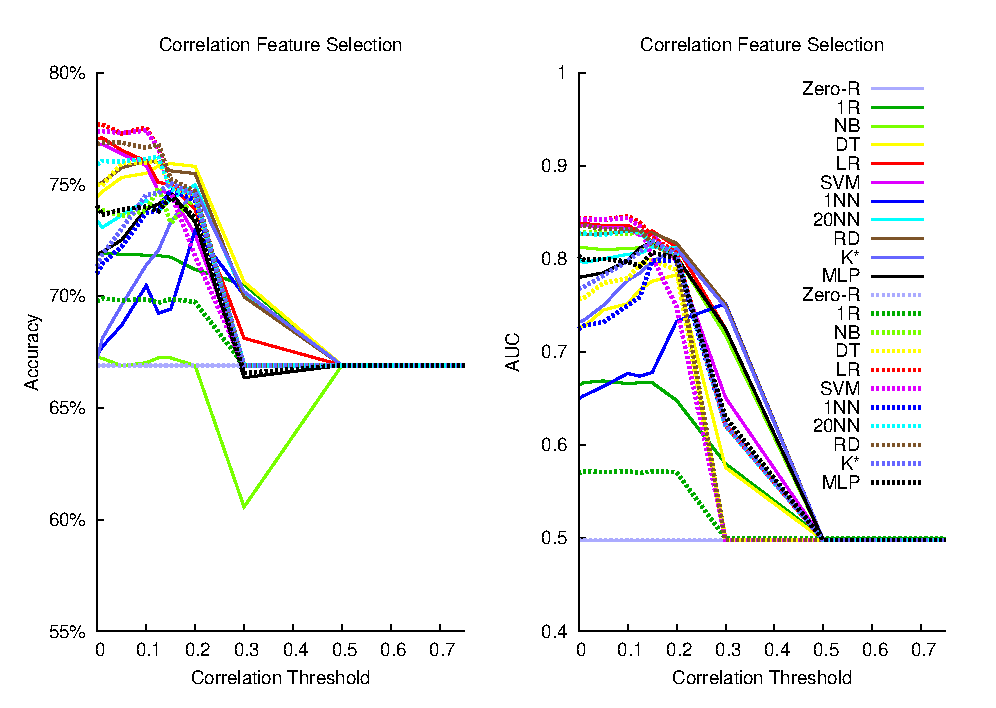
\includegraphics[width=\textwidth]{results/tr-corr.eps}
\caption{}
\label{fig:tr-threshold-corr}
\end{subfigure}

\begin{subfigure}{1.1\textwidth}
\includegraphics[width=\textwidth]{results/tr-ig.eps}
\caption{}
\label{fig:tr-threshold-ig}
\end{subfigure}
\caption[]{Comparison of accuracy and AUC between classifiers for feature selectors that discard features based on a threshold. Solid lines correspond to a result without discretisation, and dashed lines correspond to a result with discretisation.}
\label{fig:tr-threshold}
\end{figure}

Recall that in order for our work to be comparable to that of previous work on
trauma LOS prediction by Dinh et al. \cite{Dinh2013a}, we use the same data
set and also test the features they used as the baseline feature set.
From Table \ref{tab:overall-tr-acc} we can see that
the best accuracy achieved using their features is 75.06\% with logistic
regression.
It is worth noting that our best accuracy, using $k$-NN with 1
nearest neighbour, shows a statistically significant improvement of 2.75\% upon
the accuracy achieved by Dinh et al.
while using only 11 features (compared to the 19 they used). These 11 features
make up only 14.1\% of all features in the data set, and performed better than
the 11 features selected manually by the domain expert.

Despite our inclusion of accuracy as an evaluation metric, the AUC is what Dinh
et al. \cite{Dinh2013a}
used to evaluate the ability of their logistic regression classifier to
discriminate between the two LOS classes. Using their features, the best AUC
was 0.812 with logistic regression, and our best result was 0.846, also with
logistic regression. However, this was using the discretised data set with 29
features selected by correlation coefficient at a threshold of 0.1.
Although our logistic regression classifier exhibited an AUC improvement of
0.034, it required roughly 50\% more features than the baseline of 19 features.
If we are willing to sacrifice a little discriminating power, we are able to
achieve 0.838 AUC with only 11 features using the K* classifier.

Although $k$-NN with 1 nearest neighbour had the highest accuracy (77.81\%) out
of all combinations of classifiers and feature selection methods for this data
set, we should mention that logistic regression came a very close second with
77.7\%, outperforming more sophisticated approaches such as SVM and MLP. It
also achieved a higher AUC, and has the added advantages of being faster to
train and widely applied in medicine.

\subsection{Comparison of Feature Selection Methods}
The best accuracy and AUC results for
each classifier resulted from a reduced feature set obtained through a
particular feature selection method. Out of 20 combinations of classifiers
and discretisation (the 10 classifiers with and 10 without
discretisation), the C4.5 wrapper method resulted in the best
accuracy for 7 of these combinations, followed by 5 using information gain
and 4 using the correlation coefficient and very few for the other methods.
\texttt{TODO: recount the numbers in this paragraph.}

In terms of AUC, we
find that the correlation coefficient and the information gain are the feature
selectors that give the best AUC for most of the classifiers, and perform
equally well when used in conjunction with logistic regression and SVMs.
Interestingly, although the C4.5
wrapper method selects features which allow classifiers to achieve good
accuracy, only in 2 out of the 20 combinations of classifiers did it give the
best AUC result out of all the feature selectors.

Note that regardless of whether we consider accuracy or AUC to be more
important in evaluating classifiers, neither the baseline
feature set from Dinh et al. \cite{Dinh2013a} nor the features suggested by
the expert yielded better
results than automatic feature selection in all but \texttt{two?} cases. Neither
feature selection method produced the best AUC result for any classifier.
This is a surprising result because intuitively -- and in the literature -- it
has been stated that in a highly specialised field such as medicine, the domain
experts would be best-equipped to make judgements about which features to
use \cite{Witten2005}, and these should give reasonable results. However,
our results show that in attempting to classify patients according to their
LOS, we should consider both manual and automatic approaches.

Recall that $k$-NN with 1 nearest neighbour and C4.5 wrapper feature
selection produced the best accuracy (77.81\%) for the data set, and
logistic regression with correlation coefficient feature selection at a
threshold of 0.1 gave the best AUC (0.846). These two feature selection
methods selected 11 and 29 features respectively, and the features that
were chosen in common between them were: \texttt{operation}, \texttt{bp},
\texttt{iss}, \texttt{lowerlimbnopelvis}, \texttt{age}, \texttt{lowerlimbany}
and \texttt{icu}. This adds evidence to the work of Dinh et al. who found
that \texttt{iss}, \texttt{age} and \texttt{operation} were important
distinguishers of LOS $\leq$ or $>$ 2 days \cite{Dinh2013a}. We also
confirm the findings of Gabbe et al. who found that \texttt{age},
\texttt{iss} and \texttt{bp} were useful in predicting the length of
hospital stay of blunt trauma patients \cite{Gabbe2005}. Our feature
selection results also
support the findings of McGonigal et al. \cite{McGonigal1993} who used
\texttt{age} and
\texttt{iss} to predict the probability of survival for trauma patients, a
related problem in the same medical domain.
Our observations suggest the use of feature selection not only as a
pre-processing step to improve the accuracy or AUC of a classifier, but also
as a tool used independently to extract insights from medical data.

\subsection{Comparison of Classifiers}
In terms of classification accuracy, we did not find a lot of variation
between all classifiers, with Zero-R producing 66.91\% accuracy and 77.81\%
being the best we achieved -- an improvement of just over 10\%. The AUC of
the 11 classifiers we tested ranged from 0.498 with Zero-R to 0.846 with
logistic regression. Logistic regression, the \textit{de facto} method
used in LOS classification, performed consistently better than the others
across all feature
selection methods, but only when the feature set was not heavily reduced by
the feature selector: in these cases, such as the results from Figure
\ref{fig:tr-nothreshold-cfs-acc} showing classifier performance with features
selected by C4.5 and nearest
neighbour methods have higher accuracy than logistic regression. This is also
apparent from the graphs in Figure \ref{fig:tr-threshold}: for both
feature selection methods, as we increase the threshold, logistic regression
drops in performance after the initial few thresholds and is outperformed by
C4.5 and the various nearest neighbour classifiers ($k$-NN with 1 and 20
neighbours and K*), as well as our Ranked Distance algorithm.
This is true for both accuracy and AUC.

We found that in most cases, the SVM did not achieve a higher accuracy or
AUC than logistic regression with the same features even though SVMs are
considered the state-of-the-art in classification algorithms. Additionally,
as the feature set was reduced, both the discriminating ability of SVMs
(indicated by the AUC) and accuracy decreased noticeably. SVMs have not been
used in a LOS classification problem like
ours, so there will need to be further work carried out in order to assess the
suitability of using SVMs to classify patient LOS.

Although the MLP has been investigated in studies attempting to identify
factors associated with longer LOS or mortality for trauma patients
\cite{Hunter2000,McGonigal1993}, leading to improved results with the neural
network, we did not see the MLP outperform all other classifiers with respect
to accuracy or AUC for any feature selection method for this data set. In fact,
the MLP often performed no better than any of the nearest neighbour
classifiers, which use a straightfoward mechanism of classifying unseen
examples. Even if the MLP had managed to achieve superior accuracy or AUC, the
``black box'' nature of its prediction decisions is a barrier for their
widespread adoption in medical decision-making.

Nearest neighbour approaches appear to have performed well on this data set in
both accuracy and AUC, especially in comparison to more sophisticated
classifiers and when the feature set was significantly reduced. From the graphs
in Figure \ref{fig:tr-threshold}, we can see that all the nearest neighbours
approaches perform similarly when the number of features is decreased, but our
Ranked Distance algorithm showed a statistically significant improvement over
other NN algorithms. This
improvement is not apparent at smaller feature sets, where using the standard
$k$-NN algorithm with 1 or 20 neighbours performs slightly better.
The performance of NN we observed in our results is
an interesting finding because nearest neighbours have not been commonly
applied in predicting the LOS, but there is intuitive appeal in the
case-by-case nature of how these algorithms classify new examples that should
be explored further. Unlike MLPs and SVMs, prediction decision of nearest
neighbours are more transparent and understandable.

Although we were able to achieve higher accuracy and AUC than the baseline,
our best approaches also have a number of limitations which need to be pointed
out. The first point to note is that using a wrapper method of feature
selection is slower than using a filter approach (or manually picking the
features before training), as the learning algorithm used as the wrapper
needs to be invoked at each of the folds of cross-validation. Additionally,
the $k$-NN algorithm becomes slower as the data set increases in the number
of examples. We did not face such a problem during our work, but this will
need to be addressed for larger data sets. It is also common to use more
than one nearest neighbour, so care needs to be taken to find a suitable number
of neighbours for a given problem. Finally, we did not
attempt to tune the parameters of the classifiers in order to find the ones
that resulted in the best performance, so our statements are based on the
results of the default parameters of each classifier.
MLPs in particular are sensitive to
the network architecture, so it is likely that its accuracy and AUC could be
improved if the parameters were selected to optimise its performance on this
data set.

\section{Conclusions}
\label{sec:conclusions}
The best accuracy we achieved on the trauma data was 77.81\% with the $k$-NN
classifier using 1 nearest neighbour and 11 out of 78 features. This represents
an improvement over previous work done by Dinh et al. \cite{Dinh2013a}
on the same data set,
where they managed to achieve 75.06\% with logistic regression. More
importantly, we were able to improve upon their AUC of 0.812 with a result of
0.846, also using logistic regression but first discretising numeric features
and reducing the feature set to 29 features.
If we consider an even smaller number of features, then K*
gives an AUC of 0.838 with 11 features selected by the C4.5 wrapper, which
improves upon the result of Dinh et al. \cite{Dinh2013a} while using a little
more than half
the number of features. The drawback of $k$-NN and K* is that they require all
examples to be stored and then searched during classification, which becomes
storage- and computation-expensive as the data set increases in size.

An important contribution of our work is the use of several nearest neighbour
algorithms for predicting the LOS class of a patient. We found that these
techniques can achieve good accuracy and discriminating ability if a suitable
set of features is found. In addition, we proposed a new algorithm, Ranked
Distance Nearest Neighbours, which is an extension of the standard nearest
neighbours classifier that takes the relative importance
of each feature into account when determining the nearest neighbours of an
example. We found that this achieved better results than the other nearest
neighbour algorithms we evaluated, but only when most of the original feature
set was used.

Although we were able to improve on the work of Dinh et al. \cite{Dinh2013a}
and confirm the
importance of some features they and others found in predicting the LOS for
trauma patients, we did not find a single classifier or feature selector
that was superior to the others but instead observed different combinations
giving better results than others in certain situations. This highlights the
importance of understanding the data and investigating a range of classifiers
and feature selection techniques when approaching any medical data mining
problem, for which our work will become a catalogue.
However, we did find that logistic regression tended to perform well
on both data sets and across a number of feature selection methods, supporting
its common use in deriving classifiers for various medical phenomena.

\section*{Acknowledgements}

\bibliographystyle{abbrv}{
  \bibliography{../thesis/references}
}

\end{document}
